\documentclass[aspectratio=169]{beamer}
\setbeamertemplate{navigation symbols}{}
\usepackage{color,amsmath,comment, subfigure}
\usepackage{booktabs}
\def\vf{\vfill}
\usepackage{url}

%\setbeameroption{show notes}

%%%%%%%%%%%%%%%%%%%%%%%%%%
\title[]{Lecture 6: Foci}
\author[]{Matthew Salganik}
\institute[]{Sociology 204: Social Networks, Spring 2021\\Princeton University}
\date[]{
3/3: Foci and the design of technical systems

\vfill

\begin{flushleft}
\vspace{0.7in}

\includegraphics[width=0.05\textwidth]{figures/cc.png}
\end{flushleft}
}

\begin{document}
%%%%%%%%%%%%%%%%%%%%%%%%%%%
\frame{\titlepage}
%%%%%%%%%%%%%%%%%%%%%%%%%%%
\begin{comment}
\begin{frame}

SWBAT:
\begin{enumerate}
\item realize the power of edges that don't exist
\item compare psychological vs sociological explanations for network structure
\item apply the idea of foci to understand their personal networks 
\item see how sociological principles can shape the design of technical systems
\end{enumerate}

\end{frame}
\end{comment}
%%%%%%%%%%%%%%%%%%%%%%%%
\begin{frame}

\begin{center}
 
\includegraphics[width=0.9\textwidth]{figures/levy_inside_2011_title}
\end{center}

\vfill

\url{https://www.wired.com/2011/06/inside-google-plus-social/}

\end{frame}
%%%%%%%%%%%%%%%%%%%%%%%%%%
\begin{frame}

\begin{center}
 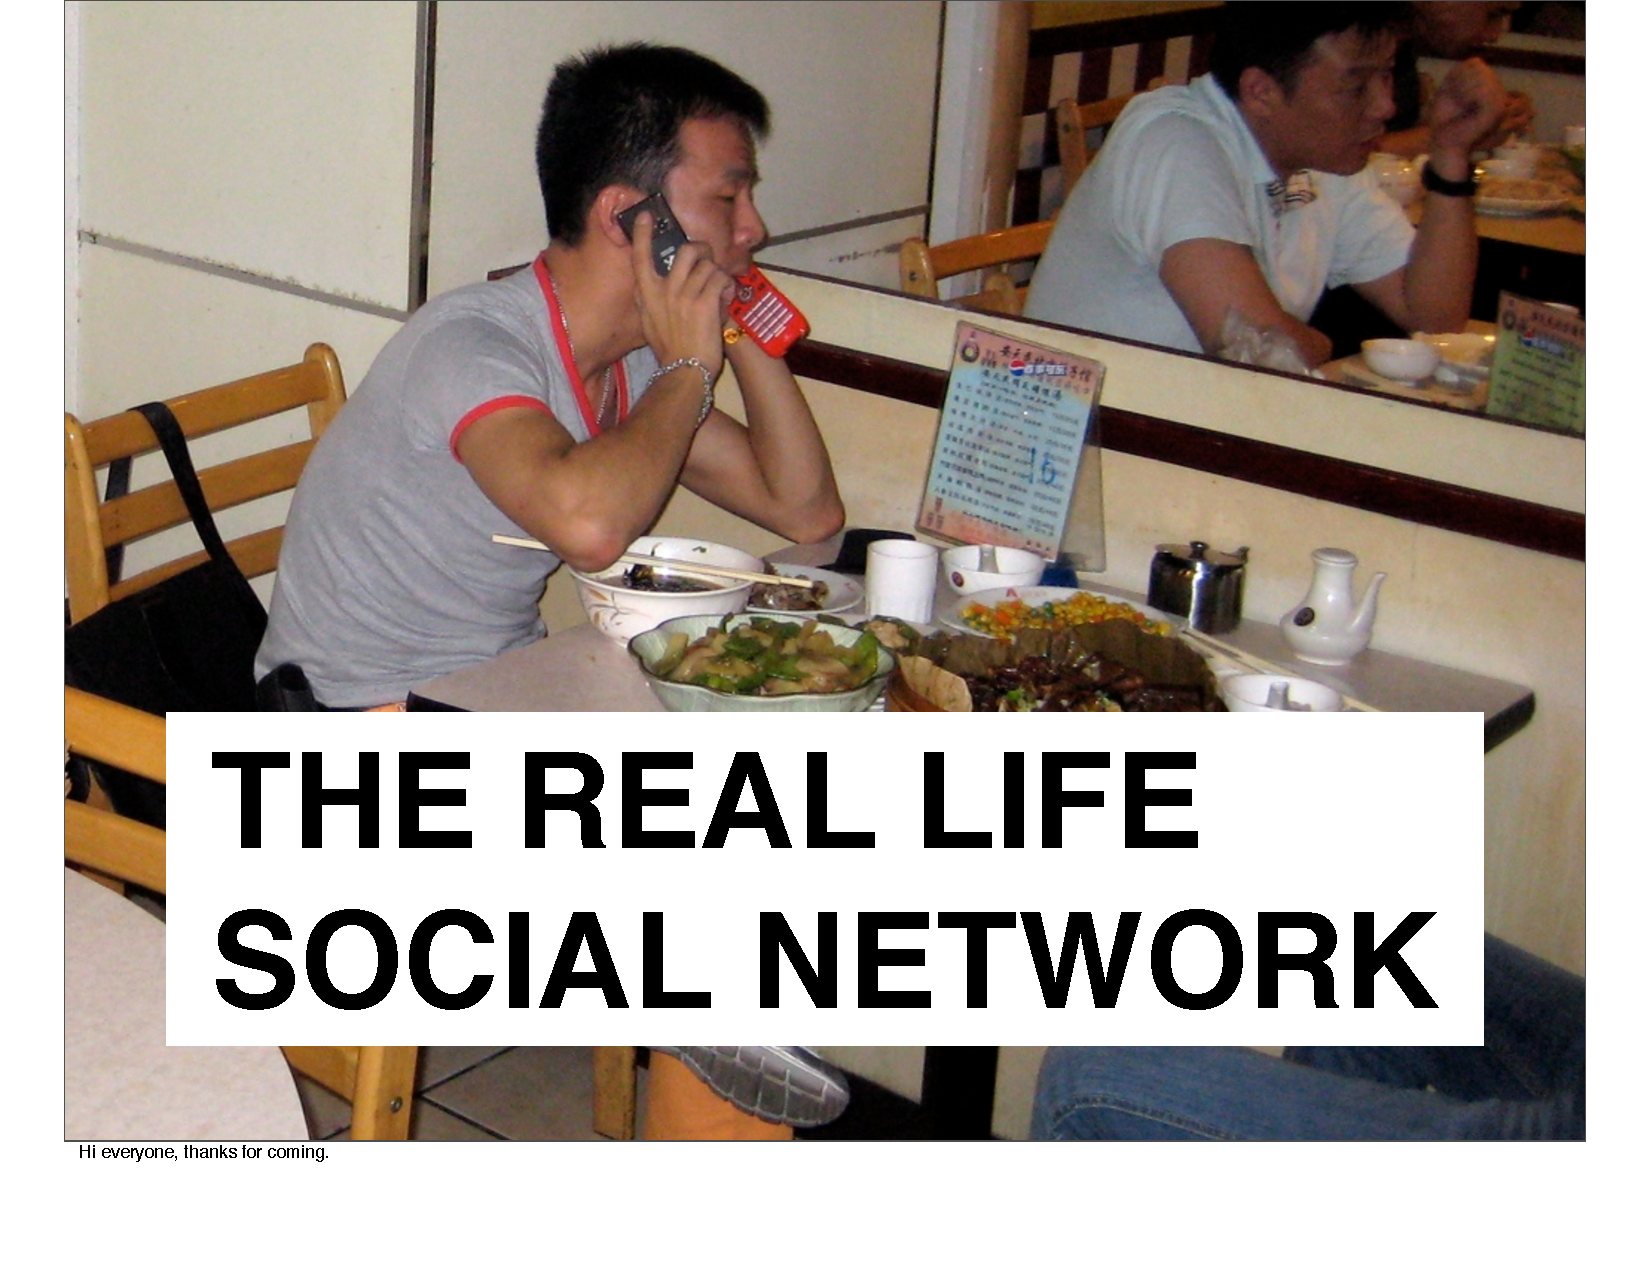
\includegraphics[width=0.65\textwidth]{figures/adams_real_2011_page1}
\end{center}

\vfill
\url{https://www.businessinsider.com/heres-the-presentation-that-inspired-google-2011-7}

\end{frame}
%%%%%%%%%%%%%%%%%%%%%%%%%%
\begin{frame}

More about Google Plus:
\begin{itemize}
\item Paul Adams \textit{Grouped: How Small Groups of Friends are the Key to Influence on the Social Web}
\item ``Google Plus: a \$585 million dollar mistake'': \url{https://slidebean.com/blog/startups-google-plus}
\item ``Looking back at Google+'': \url{https://techcrunch.com/2018/10/08/looking-back-at-google/}
\item \url{https://en.wikipedia.org/wiki/Google\%2B}
\end{itemize}

\end{frame}
%%%%%%%%%%%%%%%%%%%%%%%%%
\begin{frame}

\begin{itemize}
\item sometimes the edges that don't exist are as important as the edges that do exist
\pause
\item affiliation networks (people and groups) help us understand patterns in personal network structure
\pause
\item compare and contrast psychological vs sociological explanations for network structure 
\pause
\item sociological principles can shape the design of technical systems
\end{itemize}

\end{frame}
%%%%%%%%%%%%%%%%%%%%%%%%%%%
\begin{frame}

\begin{itemize}
\item Watts, Chapter 5. (Available from Canvas)
\item Lee, N.H. (1969). \textit{The Search for an Abortionist}: Preface, Chapter 1, and Chapter 5. (Available from Canvas). 
\end{itemize}

\note{
Recall that the Milgram experiment showed two things: 1) short paths exist and 2) people can find them.  For next class you are going to read about why people can find them.  Also, you are going to read about another kind of search: the search for an abortionist.  How would you find one if you can't google?
}

\end{frame}
%%%%%%%%%%%%%%%%%%%%%%%%%%
\begin{frame}

Please fill out the after lecture survey

\end{frame}
%%%%%%%%%%%%%%%%%%%%%%%%%%

\end{document}
